%\documentclass[aps,prb,showpacs,twocolumn,amsmath,amssymb,superscriptaddress]{revtex4-2}
\documentclass[aps,prb,showpacs,amsmath,amssymb,superscriptaddress]{revtex4-2}

\usepackage{tabularx}
\usepackage{bm}
%\usepackage[demo]{graphicx}
\usepackage{graphicx}

\usepackage{hyperref}
\hypersetup{colorlinks=true,urlcolor= blue,citecolor=blue,linkcolor= blue,bookmarks=true,bookmarksopen=false}

\usepackage{color}

\usepackage{amsmath,mathtools}
\usepackage{multirow}
\usepackage{dcolumn}
\usepackage{amssymb,amscd,xypic,bm,wasysym}
\usepackage{float}
\usepackage{cleveref}
\usepackage[caption=false,position=top,captionskip=0pt,farskip=0pt]{subfig}
\captionsetup[subfigure]{justification=raggedright,singlelinecheck=false}


\newcommand{\Red}[1]{\textcolor{red}{#1}}
%\newcommand{\vb}[1]{\boldsymbol{#1}}
\usepackage{soul}

% reset vec and hat style to a bold type
\let\oldhat\hat
\renewcommand{\hat}[1]{\oldhat{\mathbf{#1}}}
\renewcommand{\vec}[1]{\mathbf{#1}}
% stretches the vertical spacing of arrays/matrices
\renewcommand{\arraystretch}{1.5}
\setlength{\jot}{10pt}

\newcommand{\Ham}{\mathcal{H}}
\newcommand{\ke}{k_{\epsilon}}
\newcommand{\kpm}{k_{\pm}}
\newcommand{\sx}{\sigma_x}
\newcommand{\sy}{\sigma_y}
\newcommand{\sz}{\sigma_z}
\newcommand{\so}{\sigma_0}
\newcommand{\cc}{c^{\dagger}}
\newcommand{\de}{\Delta}

\begin{document}

\title{Superconducting triangular islands as a platform for manipulating Majorana fermions}

\author{Aidan Winblad}
\affiliation{Department of Physics, Colorado State University, Fort Collins, CO 80523, USA}

\author{Hua Chen}
\affiliation{Department of Physics, Colorado State University, Fort Collins, CO 80523, USA}
\affiliation{School of Advanced Materials Discovery, Colorado State University, Fort Collins, CO 80523, USA}

\maketitle

\begin{abstract}
  \Red{PLACEHOLDER**APS MM 2022 Abstract}
  We study the possibility of obtaining robust Majorana modes at the corners of triangular islands of different superconductor models, with the goal of finding alternative structures that can serve as building blocks of topological quantum computation.
  By considering both spinless p-wave and ferromagnetic Rashba s-wave superconductor models on an equilateral triangle subject to inhomogeneous supercurrents, we found that Majorana corner modes can generally appear if the system being considered can be made equivalent to a triangular chain model, which can be understood by calculating the bulk Z2 topological invariant.
  We also discussed the robustness of the corner modes in possible experimental realizations of the triangular islands.
\end{abstract}


\section{Introduction}
\Red{PLACEHOLDER}


\Red{OUTLINE: (Sec I is \dots, Sec II is \dots)}
\section{Linear vector potential effects on 1D chains}

\Red{PLACEHOLDER}

\subsection{\Red{Gap closing/reopening (Topological Change) and phase diagram}}

Recent work has predicted that placing a supercurrent along a superconducting chain can induce a topological phase change.
Another way of thinking about this is there is a constant vector potential that induces a constant phase on the hopping amplitudes on the superconducting chain.
Here we will show that using a linear vector potential can also induce a topological phase change, i.e. clsoing and reopening a gap.
\Red{Maybe here we can state the Hamiltonian in the supplementary? Explain we can't solve this analytically, thus we proceed with a numerical approach starting with the lattice space Hamiltonian.}
Let us start with the Hamiltonian of a spinless or spin-polarized $p$-wave superconductor chain
\begin{equation}
  \Ham_{ch} = \sum_j (-t\cc_{j+1} c_j + \de \cc_{j+1}\cc_j + h.c.) - \mu \cc_j c_j,
\end{equation}
where $t$ is the hopping amplitude, $\de$ is the superconducting order parameter, and $\mu$ is the chemical potential.
Next, we will apply Peierls substitution to our creation(annihilation) operators
\begin{align}
  \cc_{j+1} c_j &\rightarrow \cc_{j+1} c_j \exp \left(-\dfrac{i e}{\hbar} \int_{r_j}^{r_{j+1}} \vec{A} \cdot d\vec{l} \right) \\ \nonumber
  &\rightarrow \cc_{j+1} c_j e^{i \phi_{j+1,j}}.
\end{align}
Here the electron charge, $e$, and Planck's constant, $\hbar$, will be treated as natural numbers. The vector potential will be linear, symmetric about the y-axis, and point along the x-axis, $\vec{A} = Bx\hat{x}$ for $-L/2 \leq x \leq L/2$.
One finds that $t$ is the only term that picks up a phase, thus our modified Hamiltonian looks like
\begin{equation} \label{eq: Peierls chain}
  \Ham_{ch} = \sum_j (-t e^{i\phi_{j+1,j}} \cc_{j+1} c_j + \de \cc_{j+1}\cc_j + h.c.) - \mu \cc_j c_j.
\end{equation}

To calculate the Majorana number we need to rewrite our Hamiltonian to be in skew-symmetric form.
One such way is to write it in Majorana fermion basis, the transformation matrix is of the form
\[
  u = \dfrac{1}{\sqrt{2}} \left(
  \begin{matrix}
    1 & 1 \\
    -i & i
\end{matrix} \right)
\]
Since we are in lattice space we need to expand for the system size, we simply include a tensor product with an identity matrix of the size of the system, $U = u \otimes I_n$.
We can now arrive at the skew-symmetric matrix with the following equation
\begin{equation}
  A_{ch} = -i U \Ham_{ch} U^{\dagger}.
\end{equation}
The Majorana number, \mathcal{M}, of a 1D chain is defined as
\begin{equation}
  \mathcal{M} = \text{sgn}[\text{Pf}(A_{ch})],
\end{equation}
where $\text{Pf}$ stands for the Pfaffian of a skew-symmetric matrix.
When $\mathcal{M} = -1$, the chain is in a non-trivial topology and we would expect Majorana zero modes at the edges of a finite chain.
As we sweep through a range of $B$ values for our vector potential we expect to see a gap closing, $\mathcal{M} = 1$, and our system take on a trivial topology, thus no Majorana zero modes would exist on the edge of a finite chain.
Taking a look at figure \ref{fig: majorana-number} we can see for varying $\mu$ and $B$ values where our system is trivial and non-trivial.

\subsection{\Red{Majorana Edge modes on a double chain}}

\begin{figure}[]
  \subfloat[][]
  {
    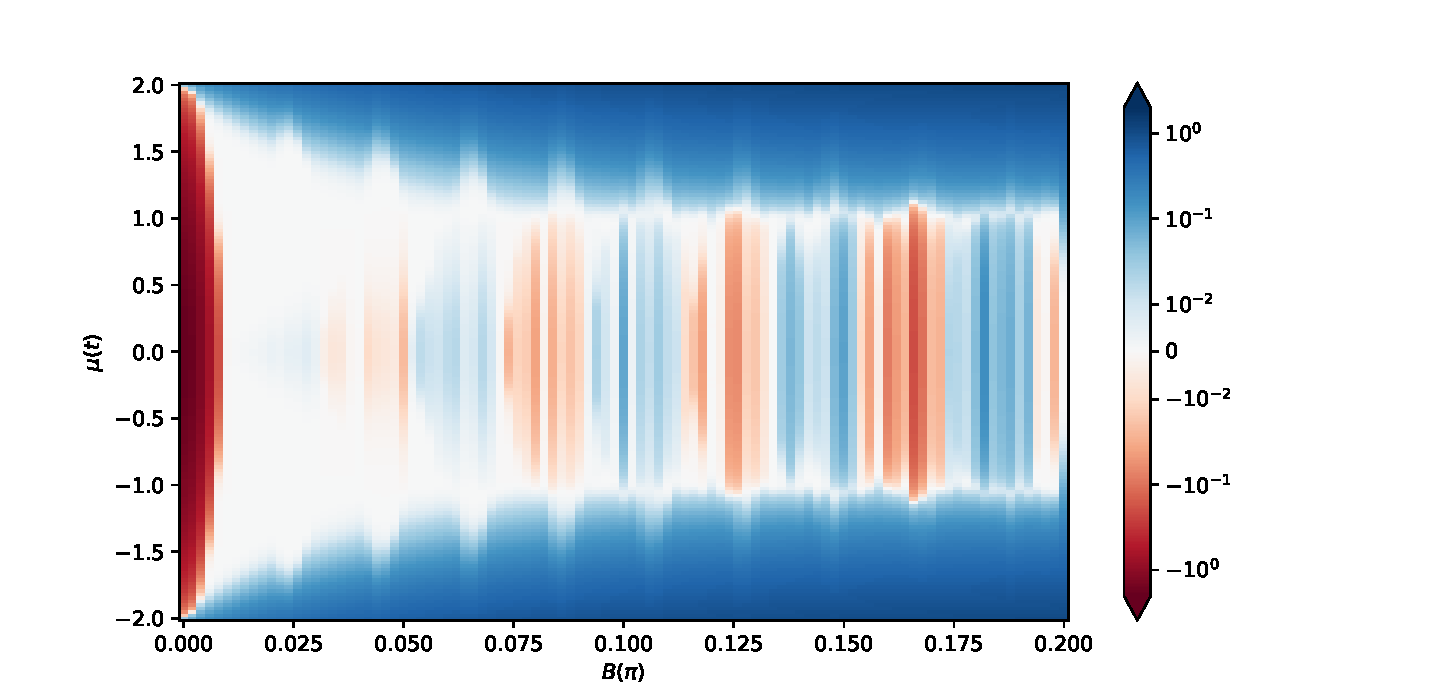
\includegraphics[width=0.34\textwidth]{./figures/linear-chain-majorana-number-full-range.pdf}
    \label{subfig:linear-chain-majorana-number}
  }
  \subfloat[][]
  {
    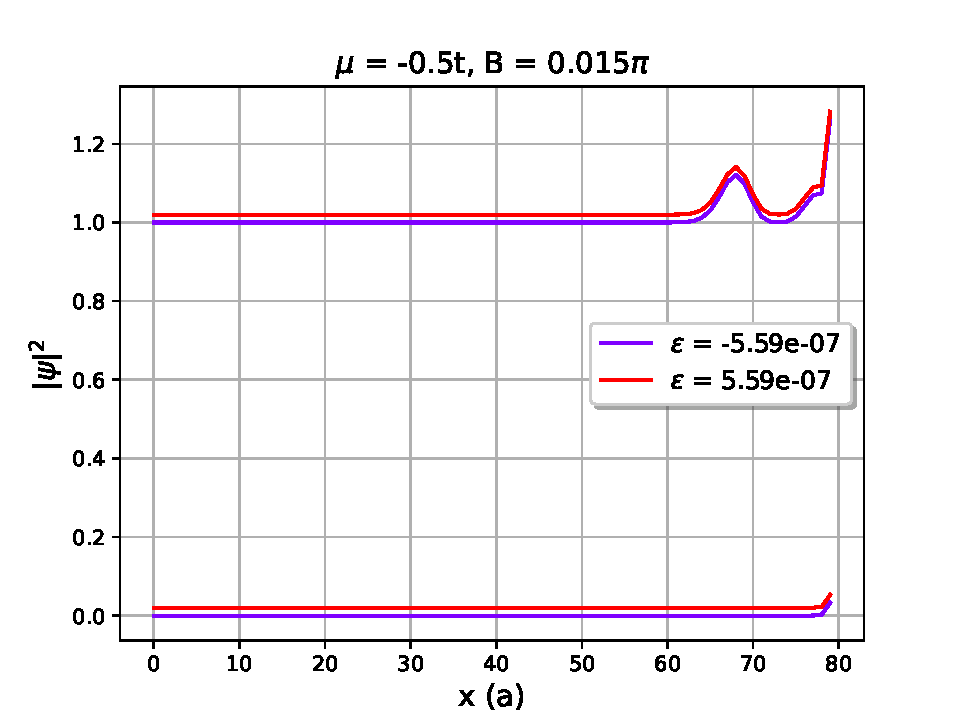
\includegraphics[width=0.22\textwidth]{./figures/double-chain-mu-n0_5-B-0_015pi.pdf}
    \label{subfig:non-trivial-double-chain-1}
  }
  \\
  \subfloat[][]
  {
    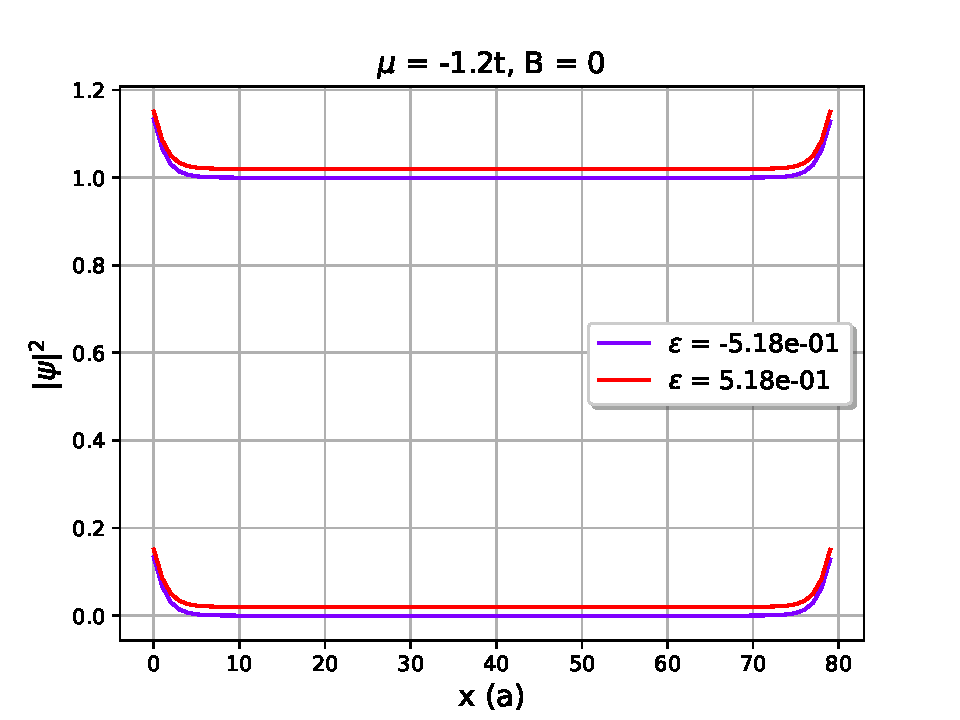
\includegraphics[width=0.22\textwidth]{./figures/double-chain-mu-n1_2-B-0.pdf}
    \label{subfig:non-trivial-double-chain-2}
  }
  \subfloat[][]
  {
    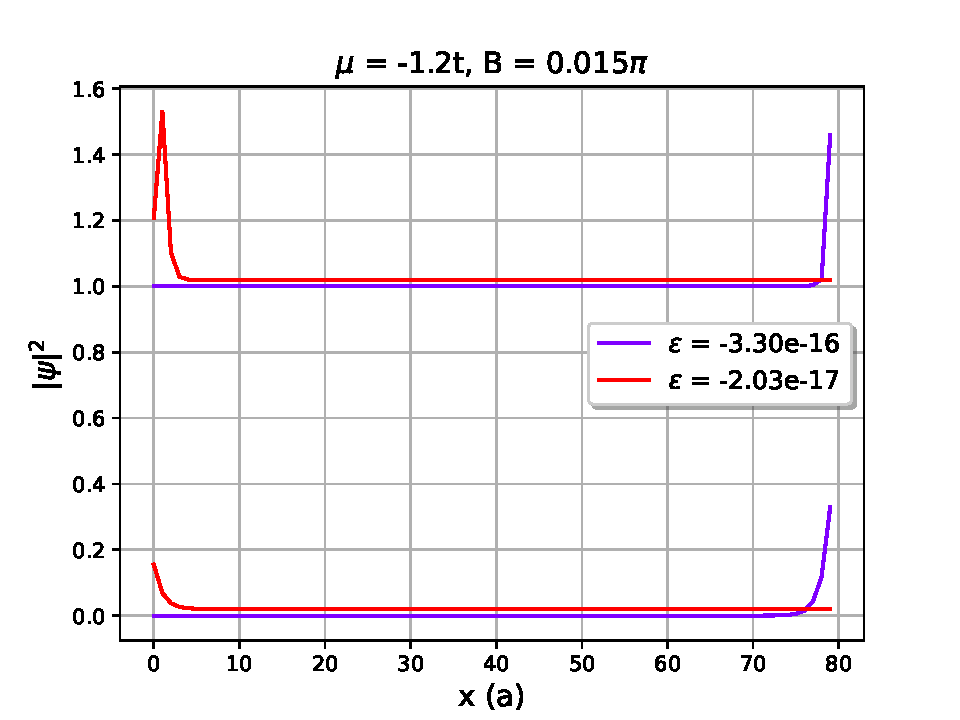
\includegraphics[width=0.22\textwidth]{./figures/double-chain-mu-n1_2-B-0_015pi.pdf}
    \label{subfig:trivial-double-chain}
  }
\caption{(a) The Majorana number is calculated for a single chain consisting of $n=80$ lattice sites with linear vector potential and parameter ranges $-2t \leq \mu \leq 2t$ and $B\leq \pi/25$. Values within the blue region tell us the chain is in a non-trivial topology, while white means it is trivial topology. (b)-(d) The eigenstates are plotted for a double chain, each chain has $n=80$ lattice sites. The top chain has an applied linear vector potential. Each chain and eigenstate are plotted with offsets for clarity: (b) $\mu=-1.2t$ and $B=0$ shows two fermion edge states at the interface (c) $\mu=-0.5t$ and $B=0.015\pi$ shows two fermionic edge states at the interface (d) $\mu=-1.2t$ and $B=0.015\pi$ shows two Majorana fermions at the interface of the two chains.}
\label{fig:majorana-number}
\end{figure}

To illustrate the importance of bulk-edge correspondence in forming Majorana fermions we take a look at two chains connected at their end points.
The top chain will have an applied linear vector potential.
Topology of the bottom chain is only determined by its chemical potential.
Both chains will be connected at the endpoints and have pairing along the y-axis.
Following figure \ref{subfig:linear-chain-majorana-number}, picking a $\mu$ and $B$ combo in the non-trivial region (blue) results in the top chain being non-trivial.
One can see in figure \ref{subfig:non-trivial-double-chain-1} and \ref{subfig:non-trivial-double-chain-2} that the connection of two non-trivial chains have no MZM's.
When we turn on the vector potential and tune the chemical potential enough like figure \ref{subfig:trivial-double-chain} we have a trivial top chain connected to a non-trivial chain resulting in MZM's at the interfaces.
Later we will use this bulk-edge correspondence in our justification of MZM's hosting on a triangular superconductor.

\section{Triangular islands}

\subsection{\Red{3-site problem and kitaev limit for tri.chain, solid triangle}}
We now expand our analysis to triangular islands.
The chain Hamiltonian in Eq. \ref{eq: Peierls chain} can be generalized as
\begin{equation} \label{eq: Peierls triangle}
  \Ham = \sum_{<j,l>} (-t e^{i\phi_{l,j}} \cc_{l} c_j + \de e^{i\theta_{l,j}} \cc_{l}\cc_j + h.c.) - \sum_j \mu \cc_j c_j,
\end{equation}
where $<j,l>$ are nearest neighbors on a triangular lattice and $\theta_{l,j}$ is the angle between the two sites.
It is difficult to come to any conclusion while in the complex fermion basis, but if we write our Hamiltonian in Majorana fermion basis we can get a clearer picture.
\Red{Maybe a see supplementary material XX for derivation here.}
The triangular Hamiltonian now takes the form
\begin{align}
  \Ham = -\dfrac{i\mu}{4} \sum_j (& a_j b_j - b_j a_j) \nonumber \\
  -\dfrac{i}{4} \sum_{<j,l>} [&(t\sin\phi_{l.j}-\de\sin\theta_{l,j}) a_l a_j \nonumber \\
  +&(t\sin\phi_{l,j}+\de\sin\theta_{l,j}) b_l b_j \nonumber \\
  +&(t\cos\phi_{l,j}+\de\cos\theta_{l,j}) a_l b_j \nonumber \\
  -&(t\cos\phi_{l,j}-\de\cos\theta_{l,j}) b_l a_j].
\end{align}
To clear things up, $\phi_{l,j} = -\phi_{j,l}$ since the direction of integration is reversed and the angle $\theta_{l,j} = \theta_{j,l} + \pi$, this ensures we have a Hermitian Hamiltonian.

Let us consider a 3-point triangle lattice, where each lattice point is a complex fermion housing two Majorana fermions.
The bottom left point will have $a_1, b_1$, bottom right has $a_2, b_2$, and the top point has $a_3, b_3$.
Similar to Kitaev we will make the same assumptions $t=\de$ and $\mu=0$.
Doing this lets us see a combination of trig terms.
We need some of these combination to go to zero.
Notice how each individual row looks like a Kitaev chain, we need to look at how the rows interact with each other.
Since our goal is to have two Majorana zero modes at the bottom corners, lets aim to have $a_1$ and $b_2$ be such modes.
Anytime $a_1$ or $b_2$ appear in our equation we need its trig terms to cancel, eliminating those particles coupling to the rest of the system.
Let us look at the energy going from site 1 to site 3, $\theta = \pi/3$, we notice the first and last term should be
\begin{align}
  a_3 a_1 (\sin\phi_{31} - \sin\pi/3) = 0, \\
  b_3 a_1 (\cos\phi_{31} - \cos\pi/3) = 0.
\end{align}
This is true if $\phi_{31} = \pi/3$.
Now let's consider the energy from site 3 to site 2.
The phase angle $\theta = -\pi/3$ and the two simplified equations involving $b_2$ are
\begin{align}
  (\sin\phi_{23} - \sin(\pi/3)) b_2 b_3 = 0, \nonumber \\
  (\cos\phi_{23} - \cos(\pi/3)) b_2 a_3 = 0. \nonumber
\end{align}
Here we see $\phi_{23} = \pi/3$.
The linear vector potential one can get with the desired phase is
\begin{equation}
  \vec{A} = \dfrac{8 \pi}{3 \sqrt{3} a^2} x \hat{y}
\end{equation}

We can now extrapulate from a 3-point triangle to a full triangular island.
The goal being to ensure Majorana zero modes at the bottom two vertices.
If instead we have a triangular island with $n_r$-many rows we find
\begin{equation}
  \vec{A} = \dfrac{8 \pi}{3 \sqrt{3} a^2} \dfrac{x}{2n_r-3} \hat{y} = Bx\hat{y}.
\end{equation}
Solving the Hamiltonian numerically we can see how turning on this Peierls phase affects the eigenenergies.
\begin{figure}[]
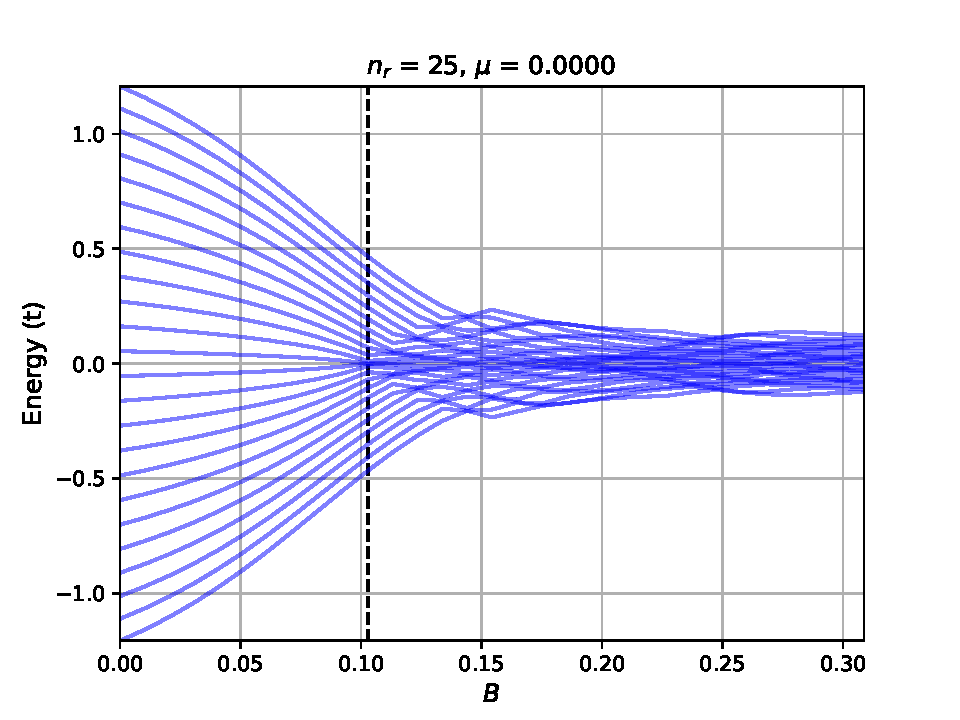
\includegraphics[width=0.5\textwidth]{./figures/nr-25-w-0-spectral-flow.pdf}
\label{fig: full-triangle-spectral}
\caption{For increasing vector potential strength MZM's appear at the critical strength, denoted with a dotted black line. Notice the density of edge states makes it unclear the Majorana zero modes live in a clean gap.}
\end{figure}

We clearly see MZM's appear at the critical, unfortunately it doesn't seem to live within a clean gap.
To get around this we instead think of using a triangular chain instead to remove a majority of the edge states.

\begin{figure}[h]
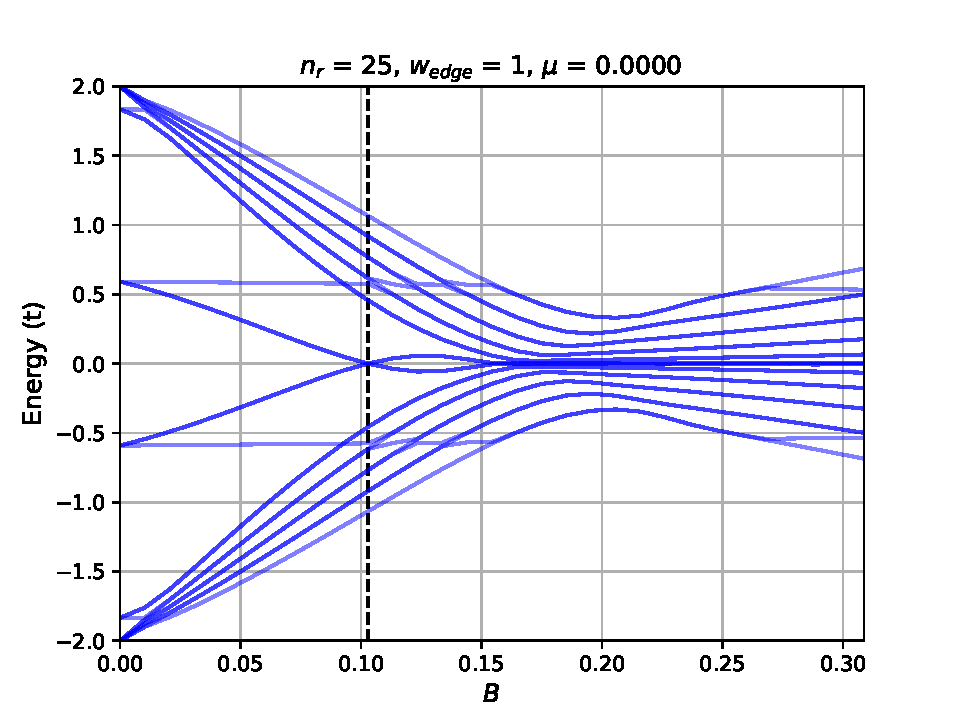
\includegraphics[width=0.5\textwidth]{./figures/nr-25-w-1-spectral-flow.pdf}
\label{fig: chain-triangle-spectral}
\caption{As the strength of the vector potential increases MZM's appear at the critical strength, denoted as the dotted black line. While a cleaner gap can be seen for the MZM's they are degenerate.}
\end{figure}
While we have effectively reduced the number of states living in the gap we see the MZM's are doubly degenerate.
This is a consequence of a triangular chain's geometry.
The next excited state becomes a zero mode due to the geometry forcing the wave function to be well separated and recombines with the other expected MZM's.
This leads us to think we should use a finite width for the sides of the triangle.

\subsection{\Red{Finite width (hollow triangle)}}

\subsubsection{\Red{Majorana number (PBC)}}

\subsubsection{\Red{Corner modes (open BC)}}

\begin{figure}[]
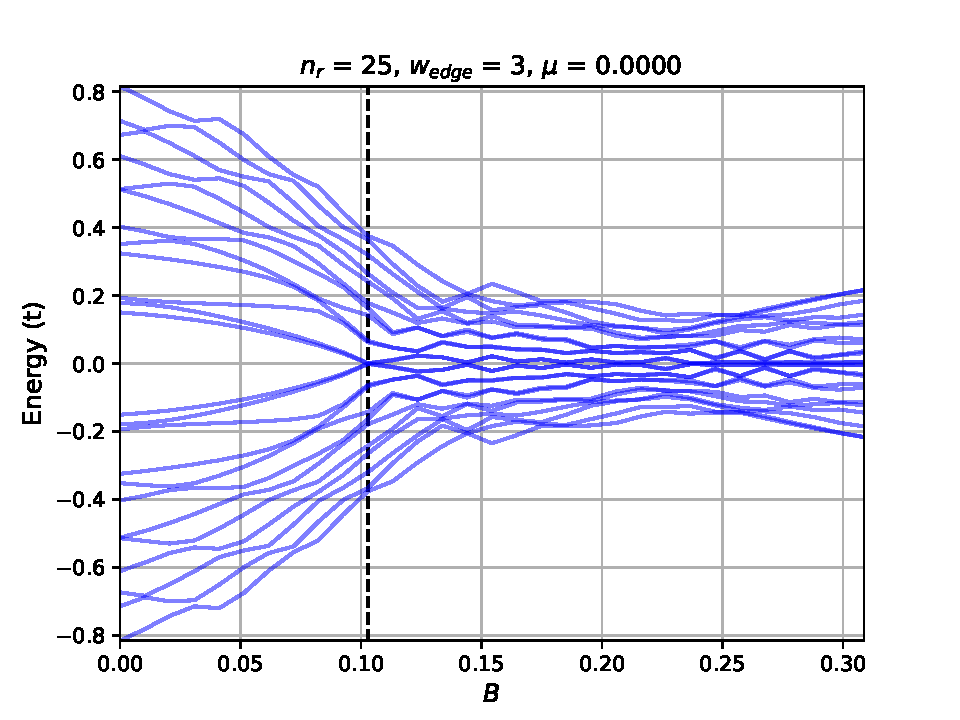
\includegraphics[width=0.5\textwidth]{./figures/nr-25-w-3-spectral-flow.pdf}
\label{fig: finite-width-triangle-spectral}
\caption{As the strength of the vector potential increases MZM's appear at the critical strength, denoted as the dotted black line.}
\end{figure}

\section{Conclusions and Discussion}

\Red{PLACEHOLDER}


\begin{acknowledgements}
  Supported by XYZ Grant No. XXXXXX etc.
\end{acknowledgements}


%\bibliography{./triag_ref}


\end{document}
